\documentclass[11pt,a4paper]{article}

\usepackage[utf8]{inputenc}
\usepackage[T1]{fontenc}
\usepackage[margin=2.5cm]{geometry}
\usepackage{graphicx}
\usepackage{booktabs}
\usepackage{array}
\usepackage{enumitem}
\usepackage{microtype}
\usepackage[hidelinks]{hyperref}

\newcommand{\sys}{AirGated}
\newcommand{\code}[1]{\texttt{#1}}

\title{\sys: A Prototype for Offline, Network-Bound Classroom Attendance\\with Device Keys and a Face-and-Blink Check}
\author{Aakshant Kumar\\
\small Department of Computer Science \& Engineering (Artificial Intelligence)\\
\small \texttt{kumaraakshant2005@gmail.com}}
\date{November 2026}

\begin{document}
\maketitle

\begin{abstract}
Attendance by roll call, QR code or GPS is defeated by cheap tricks: proxy answers, forwarded screenshots, spoofed coordinates. We describe \sys{}, a research prototype that runs with no cloud service: a host on the classroom network creates the Wi-Fi network and a captive portal, and marks a student present only if, in one request, six independent gates pass: a fresh single-use server nonce; a server-measured round trip under 20~ms; a link-layer (MAC) address matching enrollment; an RSA signature from a non-extractable browser-held key over the nonce and the submitted frames; a random-count blink liveness test; and a face match against enrollment. We report the design, a defect history from three development phases, and what the same code base needed on two hosts (a Windows Mobile Hotspot and an Ubuntu laptop access point), isolating the small operating-system-specific surface: creating the access point, resolving an IP address to a MAC address, and the start order of the DNS responder. Field evidence is small: an August test (3 of 3 check-ins accepted, mean RTT 5.5~ms), a 30~September three-student trial with 17 logged events, informal testing with at least five people, and a Linux session. A loopback load test shows that the face engine, which analyses one clip at a time (about 1.8~s each), saturates near 28 check-ins per minute well before the latency gate is affected. We propose treating a changed MAC as a re-registration trigger rather than a rejection when the device key and face still verify, and describe the next step: a dedicated, operating-system-independent access unit that bounds radio coverage to one room, removes the client cap of consumer hotspots, and lets the instructor run a class from a phone. \sys{} is a prototype, not a production system, and we list what remains before it can be.
\end{abstract}

\section{Introduction}
Attendance is a trust problem, and each common technique has a known bypass: a friend answers ``present''; a QR code on a projector is photographed and forwarded; a GPS geofence is defeated by mock-location settings; a login credential is copied to a friend's phone; a photograph of the absent student is held to a camera. \sys{} is built as layers, each meant to block one of these (Table~\ref{tab:tricks}).

The design goals are: (i) \emph{no cloud dependency} for attendance; (ii) \emph{no app installation}, only a phone browser; (iii) \emph{binding to the physical phone and the physical person}; (iv) \emph{inspectability}, with every rejection written to an audit log and shown on an instructor dashboard; and (v) \emph{independence from any particular operating system or vendor}, since the intended end state is a dedicated access unit rather than a laptop.

\begin{table}[t]
\centering
\small
\begin{tabular}{@{}p{4.6cm}p{9.6cm}@{}}
\toprule
Cheap trick & What stops it in \sys{} \\
\midrule
Friend answers ``present'' & Face must match the enrollment embedding \\
Forwarded QR code or screenshot & No QR code; each check-in signs a fresh single-use nonce \\
Fake GPS & GPS is not used; the phone must be on the classroom network with low server-measured latency \\
Logging in over a VPN or tunnel & The server times the round trip itself and rejects slow links \\
Credential copied to a friend's phone & The device key is non-extractable in the browser \\
Photo of the absent student & A random number (2 or 3) of blinks, revealed only after the nonce is issued \\
One phone checks in several students & One MAC address may check in one roll number per 60~s \\
\bottomrule
\end{tabular}
\caption{Attendance bypasses and the corresponding \sys{} control.}
\label{tab:tricks}
\end{table}

\paragraph{Contributions.}
\begin{itemize}[leftmargin=*,itemsep=2pt]
\item A six-gate check-in protocol in which the server, not the phone, measures proximity and makes every decision (Section~\ref{sec:design}).
\item A defect history from three development phases, with root causes, showing which failures were logic errors and which were ordering and environment errors (Section~\ref{sec:history}).
\item A host abstraction: five requirements any access host must meet, and the functions that were operating-system specific across a Windows and a Linux host (Section~\ref{sec:host}).
\item A treatment of per-network randomized MAC addresses that keeps the device-binding gate while not costing a forgetful student the day, with failure messages that list every mismatching check (Section~\ref{sec:mac}).
\item A loopback load test identifying the face engine as the first scaling limit (Section~\ref{sec:load}), and a concrete plan for dedicated access hardware (Section~\ref{sec:future}).
\end{itemize}

\section{Background and Related Work}
\paragraph{Local captive portals.} Phones decide whether a Wi-Fi network has internet access by requesting a known URL over plain HTTP and expecting a specific answer (for example HTTP 204). A different answer raises the OS sign-in window. \sys{} answers every DNS name with the host's address and redirects probes to its landing page until the phone has checked in. The sign-in window is a restricted web view that generally cannot open the camera, so students are sent to a full browser for the check-in.

\paragraph{MAC address randomization.} Mobile operating systems use random link-layer addresses to limit tracking; Martin et al.~\cite{martin2017mac} study how this is implemented and when it fails. Current Android and iOS releases generally use an address that is random but fixed per network, which matters for any system that uses the MAC as an identity factor (Section~\ref{sec:mac}).

\paragraph{Browser keys.} The Web Cryptography API~\cite{webcrypto} lets a key be generated non-extractable and stored in IndexedDB; page script can ask for signatures but cannot read the key. Browsers expose this API and the camera only to secure origins, so the portal must be served over HTTPS even on a closed network.

\paragraph{Relay attacks on proximity.} A rotating on-screen code resists a delayed screenshot but not a live relay: a student in the room points a camera at the projector and video-calls an accomplice, who reads the code from the live feed. Latency gating does not help, because the relay happens before any network request. We therefore treat radio containment as the primary presence boundary (Section~\ref{sec:future}). Ultrasonic proximity tokens were rejected early because attenuation rises with frequency and a laptop speaker is weak and non-directional, so back-row phones in a large room would not reliably hear it.

\paragraph{Face components.} Detection uses YuNet~\cite{yunet}, blink scoring uses face-blendshape output from MediaPipe's Face Landmarker~\cite{mediapipe}, and identity embeddings use SFace~\cite{sface} through OpenCV, with OpenCV's recommended cosine-similarity threshold of 0.363. All three models run on the host, offline.

\section{System Design}\label{sec:design}
\subsection{Architecture}
Figure~\ref{fig:arch} shows the \emph{access host}: today a laptop, later a dedicated unit. It provides the Wi-Fi network and DHCP; a DNS responder that answers every query with the host's address; a plain-HTTP listener for OS probes, the landing page and the classroom certificate; and an HTTPS application (FastAPI) serving the portal, a challenge WebSocket, the registration and check-in APIs, and the instructor dashboard. State is kept in SQLite (registry, attendance records, audit log). The face engine and the neighbour table are reachable only from the application.

\begin{figure}[t]\centering
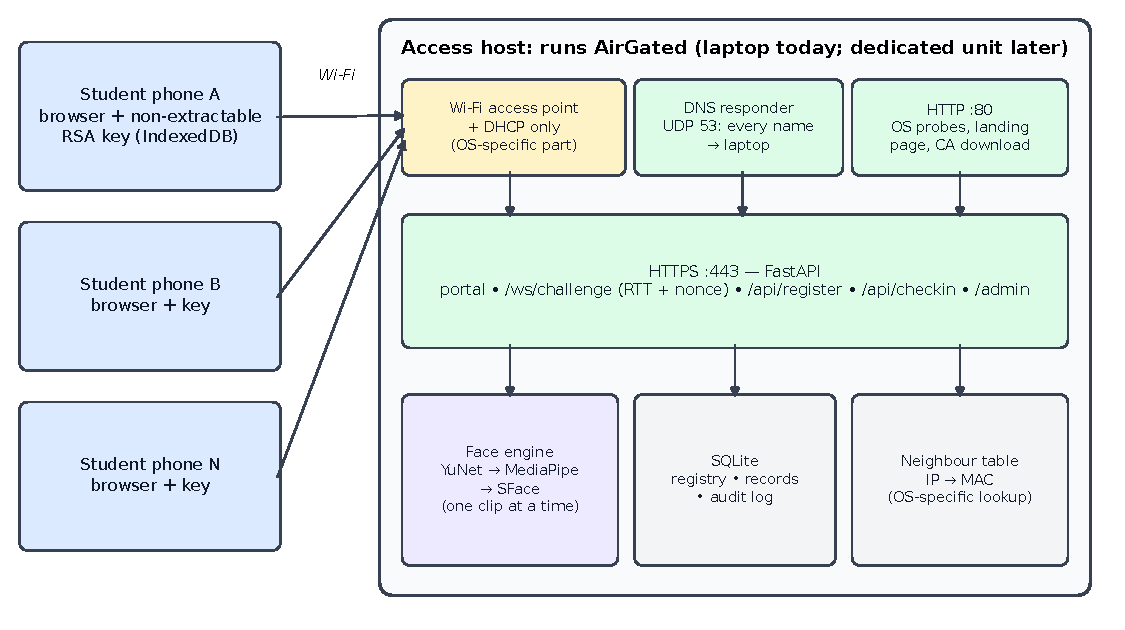
\includegraphics[width=0.95\linewidth]{figures/fig_architecture.pdf}
\caption{Architecture of the access host. Only the access point/DHCP block is tied to the operating system's network stack.}
\label{fig:arch}
\end{figure}

\subsection{Enrollment}
The browser generates an RSA-2048 key (RSASSA-PKCS1-v1.5, SHA-256) as non-extractable, requests a challenge, records a short clip while the student blinks, and signs the canonical message below with the new key as proof of possession. The server verifies the signature against the submitted public key, runs liveness, derives the face embedding (mean of up to 12 eyes-open frames, each required to be consistent with the mean), reads the MAC from its neighbour table, and stores key, MAC and embedding. The private key is persisted by the browser only after the server accepts, so a rejected enrollment leaves no orphaned key.

\subsection{Challenge and signed message}
Each registration or check-in consumes exactly one server-issued challenge: a 128-bit random nonce bound to purpose, roll number and client IP, valid for 120~s and deleted on first use. It carries the server-measured RTT and a random blink count $K\in\{2,3\}$, revealed only after the nonce is issued. The phone signs
\begin{center}\small\code{airgated|<purpose>|<nonce>|<roll>|<sha256(frames)>}\end{center}
where the last field is the SHA-256 digest of the concatenated JPEG frames, so neither the nonce nor the video can be swapped after signing.

\subsection{The check-in gates}
Figure~\ref{fig:checkin} shows the pipeline. The latency gate uses the \emph{minimum} of ten timed pings after three discarded warm-up pings. Phones in Wi-Fi power save wake only about every beacon interval ($\approx$100~ms), so some pings are slow even beside the access point; congestion and sleep can only slow a ping, while a tunnel cannot make its fastest ping quicker than its real path. The threshold is 20~ms. The face gate requires one face in at least 60\% of frames, at least $K$ blinks (open$\to$closed$\to$open with hysteresis at 0.25/0.45 on the mean eye-blink score), and cosine similarity $\ge 0.363$ to the enrolled embedding. Every rejection is written to an audit table with event, roll number, IP, MAC and detail.

\begin{figure}[t]\centering
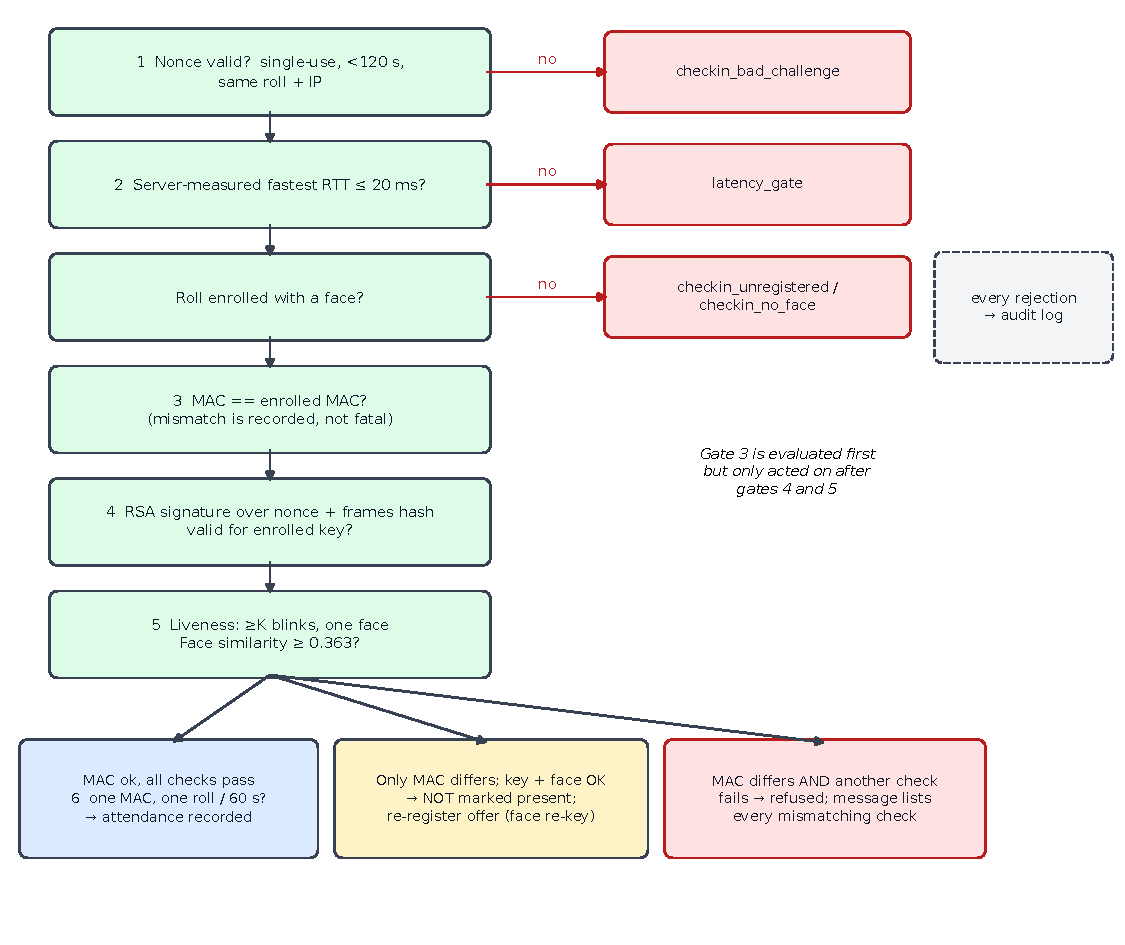
\includegraphics[width=0.85\linewidth]{figures/fig_checkin.pdf}
\caption{Check-in pipeline. A MAC mismatch is recorded at gate 3 but acted on only after the key and face checks, so a changed MAC alone leads to a re-registration offer instead of a rejection (Section~\ref{sec:mac}).}
\label{fig:checkin}
\end{figure}

\subsection{Enrollment lifecycle}
Early versions silently overwrote whichever roll was registered to a MAC, which downgrades the model to ``trust the latest device on this MAC''. The rules are now explicit: a device already enrolled to a different roll is refused (one phone, one student); a new roll enrolls normally; a roll already enrolled with a face re-keys to a new phone only if the new face matches the stored one (audit event \code{reenroll\_device}); a mismatching face is refused; and the instructor can reset a lost or replaced phone, which is audit-logged.

\section{Roles and User Flows}\label{sec:roles}
\sys{} has three roles. The \emph{student} needs only a phone browser. The \emph{instructor} starts and observes a session and handles exceptions. An \emph{institution administrator} (not implemented) would manage rooms, retention and reporting.

\paragraph{Student.} Figure~\ref{fig:student} shows the flow: join the class network, enroll once (roll number, name, blink at the camera), then check in each class. A check-in ends in one of three ways: present, refused with a message naming every mismatching check, or an offer to re-register when only the MAC has changed. Re-registration needs a fresh face match and then a normal check-in.

\begin{figure}[t]\centering
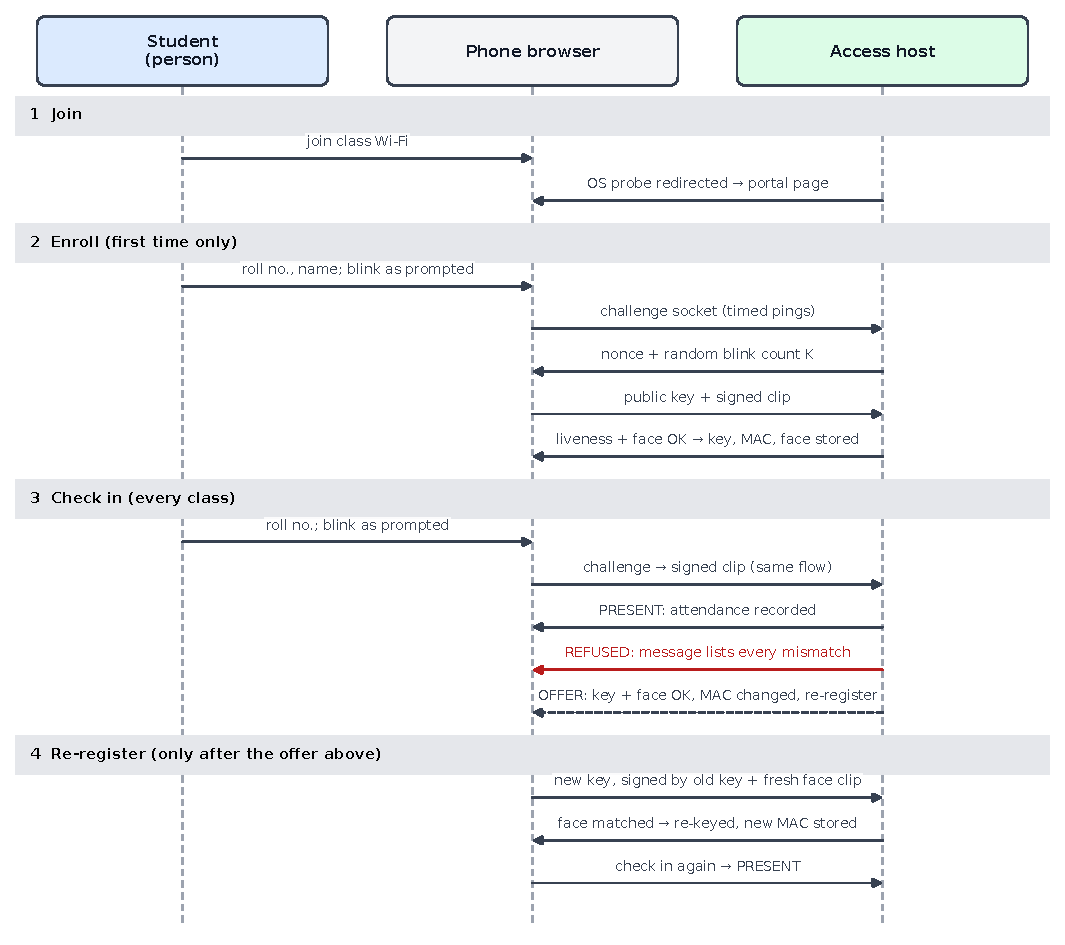
\includegraphics[width=0.85\linewidth]{figures/fig_student.pdf}
\caption{Student flow. The re-registration offer appears only when the device key and face verified and the MAC differs.}
\label{fig:student}
\end{figure}

\paragraph{Instructor.} Figure~\ref{fig:instructor} shows the flow. In the prototype the dashboard (present and absent lists, failure reasons by count, a seven-day trend, and a ``needs attention'' list of students who failed and were never marked present) is served only to the host itself, a security choice that also means the instructor must sit at the host. The dashed message in the figure, opening the dashboard from the instructor's own phone, is \emph{proposed}: it needs an authenticated instructor channel, for example the instructor's phone enrolled with its own non-extractable key and the same face check, plus a rate limit. We have not built it.

\begin{figure}[t]\centering
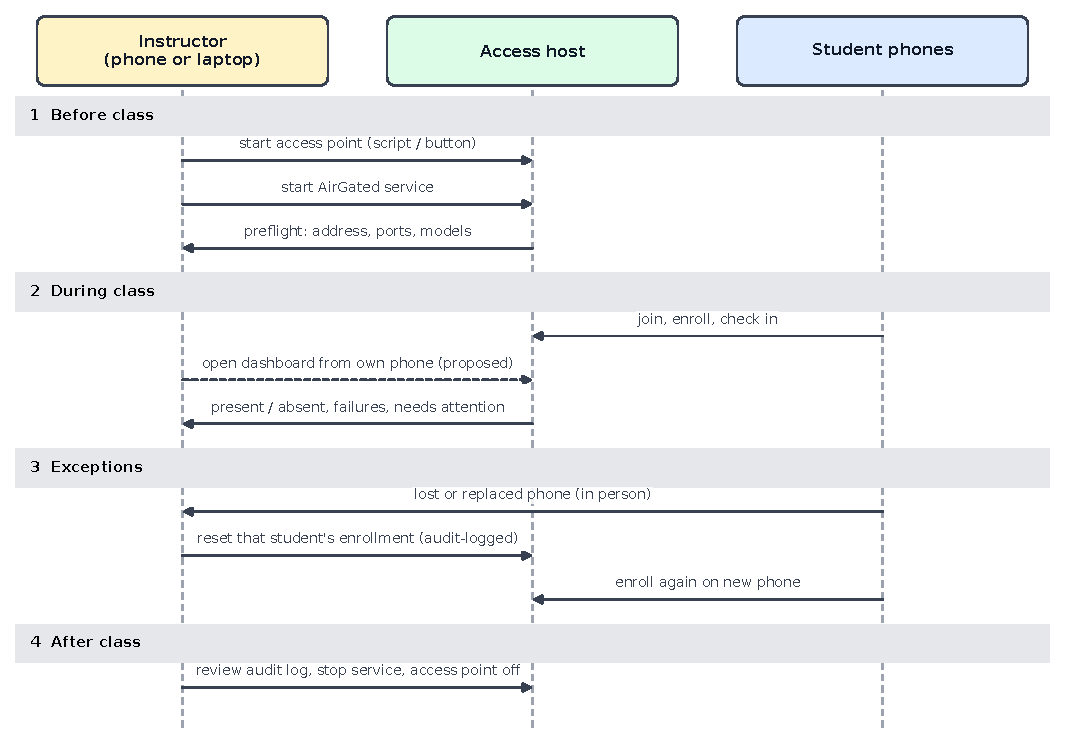
\includegraphics[width=0.85\linewidth]{figures/fig_instructor.pdf}
\caption{Instructor flow. The dashed arrow (dashboard from the instructor's phone) is proposed, not implemented.}
\label{fig:instructor}
\end{figure}

\section{Engineering History and Defects}\label{sec:history}
The system went through three phases. The first used a cloud endpoint and browser geolocation with a Haversine distance, abandoned because client-side GPS is trivially spoofed. The second bound each phone to a browser-held key. The third hardened the network layer and added the face and blink gate. The defects found along the way are instructive because most were not logic errors (Table~\ref{tab:defects}).

\begin{table}[t]
\centering
\small
\begin{tabular}{@{}p{3.6cm}p{4.9cm}p{5.4cm}@{}}
\toprule
Defect & Root cause & Fix \\
\midrule
Private key exportable & The live inline portal generated the key with \code{extractable: true} and kept it in \code{localStorage}; the correct template was dead code & Non-extractable key in IndexedDB, saved only after server acceptance \\
\addlinespace
Every registration and check-in returned \code{null} & A catch-all route was registered before the API routes; a bare \code{return} in a matched route sends an empty body & Register the catch-all last; regression test \\
\addlinespace
No OS sign-in popup & Port-80 listener answered every probe with 204, the ``internet works'' answer & Redirect probes until the phone has checked in \\
\addlinespace
DNS responder failed to start (Windows) & Internet Connection Sharing binds UDP 53 when the hotspot is switched on & Start the server first, then the hotspot \\
\addlinespace
Replayable check-ins & Challenge was a hard-coded constant & Single-use server nonce, signature covers the frames \\
\addlinespace
Spoofable latency & Phone reported its own RTT; only the last of three pings was timed & Server times ten pings after three warm-ups, uses the minimum \\
\addlinespace
MAC unresolved on a home router & AP isolation stops client-to-client traffic, so the neighbour table is never populated & Requirement: the host must be the network's gateway (Section~\ref{sec:host}) \\
\addlinespace
Silent re-binding & Re-registering overwrote the stored owner of a MAC & Face-matched re-key, one phone per roll, audited \\
\bottomrule
\end{tabular}
\caption{Defects found and their root causes.}
\label{tab:defects}
\end{table}

Three of these (route order, the port-53 race and the AP-isolation dependency) were ordering or environment failures that produced no visible error, which is why every rejection is now audit-logged with a typed reason. The test suite exercises the real application in memory (HTTP and WebSocket) with a temporary database; each simulated phone owns a real RSA key and signs in the browser's exact format, and the face engine is replaced by a stub so tests choose what the camera ``sees''. To check that the tests detect defects, five bugs were injected into a throwaway copy (nonce not deleted after use, face check removed, blink counter incrementing by two, probes answered 204 for everyone, MAC comparison disabled); all five were detected. The suite is now 34 tests.

\section{The Access Host: Requirements and Two Instantiations}\label{sec:host}
Moving the system from a Windows laptop to an Ubuntu laptop exposed exactly which parts depend on the host. Everything else (routes, gates, face engine, database, dashboard) ran unchanged. We summarise this as five requirements:
\begin{enumerate}[leftmargin=*,itemsep=1pt,label=\textbf{H\arabic*}]
\item \textbf{Gateway and no client isolation.} The host must be the network's layer-2 gateway; otherwise it cannot see the phone's MAC.
\item \textbf{Owned DNS and DHCP.} It must answer every DNS name with its own address and hand out leases that name itself as gateway and resolver, with no second DNS or DHCP service competing.
\item \textbf{Privileged ports.} It must bind UDP 53 and TCP 80 and 443.
\item \textbf{Neighbour-table access.} It must resolve a client IP to its MAC.
\item \textbf{Stable address.} Its address on the class network must exist before the DNS responder binds, or the responder must bind a wildcard address.
\end{enumerate}

\begin{table}[t]
\centering
\small
\begin{tabular}{@{}p{2.6cm}p{5.5cm}p{5.8cm}@{}}
\toprule
Requirement & Windows (Mobile Hotspot) & Ubuntu (NetworkManager AP) \\
\midrule
Access point + DHCP & Provided by the OS (ICS) at \code{192.168.137.1}; capped at 8 clients by default & Created with \code{nmcli}; DHCP-only \code{dnsmasq} (\code{port=0}) so it does not own DNS \\
\addlinespace
DNS responder & ICS binds UDP 53 when the hotspot starts, so start the server first & \code{systemd-resolved} holds 53 on loopback; bind \code{0.0.0.0} or the hotspot address, so the hotspot must exist first \\
\addlinespace
IP to MAC & \code{arp -a} & \code{/proc/net/arp}, falling back to \code{ip neigh}; \code{arp} is not installed by default \\
\addlinespace
Privileged ports & Administrator & Root or a lowered unprivileged-port floor \\
\bottomrule
\end{tabular}
\caption{The operating-system-specific surface. The order of starting the hotspot and the server is reversed between the two.}
\label{tab:os}
\end{table}

Table~\ref{tab:os} lists how each requirement was met. On Linux the port was done without editing the Windows entry point: a launcher imports the application and replaces two functions (IP-to-MAC lookup and the DNS responder), and a script creates the access point; all 31 original tests passed unchanged. Two Linux findings generalise. First, NetworkManager silently converted \code{ipv4.method manual} to \code{shared} for access-point profiles, which started its own \code{dnsmasq} on ports 53 and 67 and would have blocked the DNS responder; only reading the stored profile back and noticing \code{DHCP, IP range 192.168.137.10 -- .254} in the journal revealed it. Only \code{disabled} is kept, so the address is added directly. Second, phones initially failed to join with the correct password; the journal changed from silence to \code{AP-STA-POSSIBLE-PSK-MISMATCH} after the WPA2/WPA3 transition mode was removed, and joining then worked after the saved network was forgotten and a simple password retyped. We did not isolate which of the two changes cured it.

Because the Linux card serves as the access point, the laptop has no internet while a session runs; attendance does not need it. The Windows cap of 8 clients can be raised by a registry override on paper, but the radio and driver still limit it in practice, and one student's whole flow (associate, lease, key generation, pings, sign, upload) took 15--30~s in early tests, so cycling a class of 67 through 8 slots would take over ten minutes even in the best case. The Linux driver reports no station limit (\code{iw list} prints none), which does not prove there is none; we have not measured it.

\section{Field Evidence}\label{sec:eval}
All evidence is small; none of it supports estimates of error rates.

\paragraph{August test (Windows).} A phone never seen by the network joined without configuration, was redirected by the OS sign-in window, enrolled, and checked in three times: 3 of 3 accepted, server RTT 6.00, 5.01 and 5.44~ms (mean 5.48~ms), the MAC stable across the three requests.

\paragraph{30 September trial (Windows).} Three students on their own phones about one metre from the host produced 17 logged events: 3 enrollments, 4 accepted check-ins and 10 rejections (Table~\ref{tab:sep}). The MAC gate stopped a check-in sent from another student's phone; a face that did not match scored 0.204 against genuine scores of 0.715--0.879.

\begin{table}[t]
\centering
\small
\begin{tabular}{@{}p{6.2cm}p{7.8cm}@{}}
\toprule
Observation & Value \\
\midrule
Genuine face similarity (accepted) & 0.715--0.879 \\
Impostor face similarity (rejected) & 0.204 (threshold 0.363) \\
RTT of accepted check-ins & 3.9--7.2~ms \\
Latency false rejections (median-of-five estimator) & 2 of 12 attempts (212.9~ms and 25.3~ms) \\
Liveness false rejections & 4 of 12 check-ins, 2 of 5 enrollments \\
Cross-device check-in & Rejected by the MAC gate \\
\bottomrule
\end{tabular}
\caption{30 September 2026 trial. Three genuine and one impostor sample are far too few to calibrate thresholds.}
\label{tab:sep}
\end{table}

The two latency rejections occurred at about one metre, where propagation cannot explain 212.9~ms; power save did, and led to the minimum-of-ten estimator. Liveness rejections were the dominant friction: the blink counter saw fewer blinks than requested, plausibly because sampling at about 12~fps leaves a blink's closed phase in one to three frames, a single blurred frame can stay below the closed threshold, and students begin blinking during the countdown.

\paragraph{Wider testing.} The author also tested with at least five people overall. Only logged sessions are reported as data.

\paragraph{Linux session (5 November 2026).} The same application served two phones from the Ubuntu access point; one student's check-in, re-registration and later check-in appear in Section~\ref{sec:mac}.

\section{Randomized MAC Addresses and the Device-Binding Gate}\label{sec:mac}
After moving to the Linux access point, a previously enrolled student failed the MAC gate. The log contained the enrolled address \code{36:59:ce:63:d1:b8} (the locally administered bit is set, so it is a random address) and, on the new network, either the phone's real address (\code{00:9c:c0:...}) or a different random one (\code{e6:4d:43:...}).

\paragraph{Observation.} Over six phones and three to four days on the Windows hotspot, with no MAC-related setting changed, each phone kept the same address on a given network until it forgot the network; on Linux one phone presented the same random address across repeated check-ins. We therefore treat the address as stable per network, changing when the network name changes or the network is forgotten. This was informal and uninstrumented, on one class of devices. An earlier report had predicted random addresses would change between reconnects and listed disabling private addresses as a deployment prerequisite; the observation weakens that concern, though it does not exclude rotation after OS updates.

\paragraph{Problem.} Rejecting at gate 3 before checking the key and face made a forgotten network cost a student the day, and the message (``Hardware MAC address signature mismatch'') said nothing about what to do.

\paragraph{Change.} A MAC difference no longer ends the check-in; the signature and the face and blink analysis still run. If only the MAC differs, attendance is \emph{not} marked, the server logs \code{mac\_changed\_verified}, and the page offers re-registration, which reuses the face-matched re-key path. If the MAC differs and anything else fails, the check-in is refused with a message that lists every mismatching check, for example ``Not matching: 1. Wi-Fi hardware (MAC) address differs ... 2. Face does not match the enrolled student'', and no re-registration is offered. If the MAC matches, behaviour is unchanged. A valid signature from a non-extractable key shows the enrolled browser is answering, and the face match shows the enrolled person holds it, so a changed address alone is not evidence of fraud. The MAC still drives the 60-second one-phone-one-student gate. The cost is that the MAC is no longer a hard factor; this is a trade-off whose rationale is that the key and face already bind the phone and the person.

\paragraph{Live confirmation.} The audit log recorded \code{mac\_changed\_verified} (face 0.674), a failed re-registration (asked for 2 blinks, saw 0), \code{reenroll\_device} (face 0.618), then an accepted check-in (face 0.582, three blinks, RTT 3.7~ms), all above the 0.363 threshold. Four new tests cover the verified, wrong-face, foreign-key and too-few-blinks cases.

\section{Load Test}\label{sec:load}
The latency gate and the face engine are the two components most likely to degrade in a full class. A load test starts a private server on loopback with a scratch database and inserts fake enrollments. $N$ simulated students each open the challenge WebSocket (answering pings), wait one second, and post 62 frames of a real face photograph (15~KB each) with a valid signature, starting over three seconds. Because the frames are a still image, liveness fails \emph{after} the full face analysis, so CPU cost approximates a real check-in (detection, blendshapes and up to 12 embeddings) while recording no attendance. Over loopback the RTT is near zero, so any RTT reported is delay from the server being busy. The machine had 20 logical CPUs and 14~GB of memory.

\begin{table}[t]
\centering
\small
\begin{tabular}{@{}rccccc@{}}
\toprule
$N$ & RTT p95 / max (ms) & Gate rejections & Response p50 (s) & Response p95 (s) & Check-ins/min \\
\midrule
1 (lone)  & 0.6 / 0.6 & 0/1  & 2.2 & 2.2  & 11.1 \\
5         & 0.4 / 0.4 & 0/5  & 3.7 & 6.4  & 28.3 \\
10        & 0.7 / 0.9 & 0/10 & 9.8 & 16.7 & 27.9 \\
\bottomrule
\end{tabular}
\caption{Loopback load test; one run per level. An unqueued analysis takes 1.81~s.}
\label{tab:load}
\end{table}

The latency gate was unaffected (maximum RTT 0.9~ms against 20~ms) because analysis runs in worker threads while the event loop keeps answering pings. Response time grows with queue depth and throughput saturates near 28 per minute. The cause is a global lock around the face engine: one clip is analysed at a time. A 1.81~s analysis bounds throughput at about 33 per minute, close to the measured 28. If this holds at larger $N$, which we did not measure, 60 students arriving together would queue for about two minutes. The nonce is consumed at the start of the request, before analysis, so queueing does not expire it, but the student waits that long for an answer. The test cannot measure radio airtime or the access point's station limit; a monitor script that logs associated stations, leases, per-device ping times and check-in RTTs per interval is provided for use with real devices.

\section{Threats and Limitations}\label{sec:limits}
\begin{itemize}[leftmargin=*,itemsep=2pt]
\item \textbf{Sample sizes.} The instrumented Windows trial had three students (17 events) and the Linux session two phones. The 0.363 threshold is the library default, not calibrated on this population. The six-phone MAC observation is informal.
\item \textbf{Liveness.} Replaying a video of the student blinking the requested number of times into the enrolled phone's camera is not defeated by blink counting; a randomized head-turn challenge is the planned countermeasure. Blink false rejections are the main usability problem.
\item \textbf{Presence is network membership.} Wi-Fi reaches corridors and neighbouring rooms, and the latency gate cannot see distance within radio range. A student in the corridor passes it; the face check shows who holds the phone, not where.
\item \textbf{Weaker MAC factor.} Section~\ref{sec:mac} deliberately lets a MAC change pass when key and face verify.
\item \textbf{Capacity.} The Linux access point's station limit is unmeasured and the load test covers 10 concurrent check-ins on loopback.
\item \textbf{State and privacy.} Nonces are held in memory; the dashboard relies on loopback-only access; face embeddings and evidence photographs are stored with no automatic deletion or consent screen; there is no rate limiting on challenges.
\item \textbf{Host trust.} The host holds the registry and all decisions; compromise of the host compromises the class's records.
\end{itemize}

\section{Prototype Status and Path to Production}\label{sec:status}
\sys{} is a prototype. The pipeline is complete and tested for a single room, but ``works in trials'' is not ``ready for production'', and turning the first into the second needs time and measurements that have not been made. Table~\ref{tab:readiness} separates what exists from what is missing. We make no schedule claim.

\begin{table}[t]
\centering
\small
\begin{tabular}{@{}p{3.2cm}p{4.9cm}p{5.8cm}@{}}
\toprule
Area & Current state & Needed before production use \\
\midrule
Liveness & Blink count at about 12~fps; high false rejection in the September trial & Log per-frame scores, calibrate, raise capture rate, add head-turn challenge \\
\addlinespace
Face threshold & Library default 0.363 & Genuine and impostor distributions from the real class under room lighting \\
\addlinespace
Room presence & Network membership only & Radio containment and a site survey per room (Section~\ref{sec:future}) \\
\addlinespace
Capacity & Face analysis serialized, about 1.8~s per clip; station limit unmeasured & Parallel or accelerated face pipeline; measured client limit with real phones \\
\addlinespace
Instructor access & Dashboard on the host only & Authenticated instructor access from a phone, rate limiting \\
\addlinespace
Data protection & Embeddings and photos kept indefinitely & Consent, retention and deletion policy; encryption at rest \\
\addlinespace
Operations & Manual startup and scripts; single room & Appliance packaging, updates, multi-room management, monitoring \\
\addlinespace
Assurance & 34 tests, mutation checks, few live trials & Security review; trials at class scale (60+ students) across phone models and OS versions \\
\bottomrule
\end{tabular}
\caption{What the prototype has and what a production system still needs.}
\label{tab:readiness}
\end{table}

\section{Future Work: Dedicated Access Hardware}\label{sec:future}
Both hosts so far are borrowed machines. A Windows hotspot caps clients and owns UDP 53; a Linux laptop uses its only radio for the access point and goes offline. Neither controls where the signal goes. The next step is a purpose-built access unit running an operating-system-independent service, with the aim of controlling the \emph{area} the radio covers and the \emph{direction} it points.

\begin{figure}[t]\centering
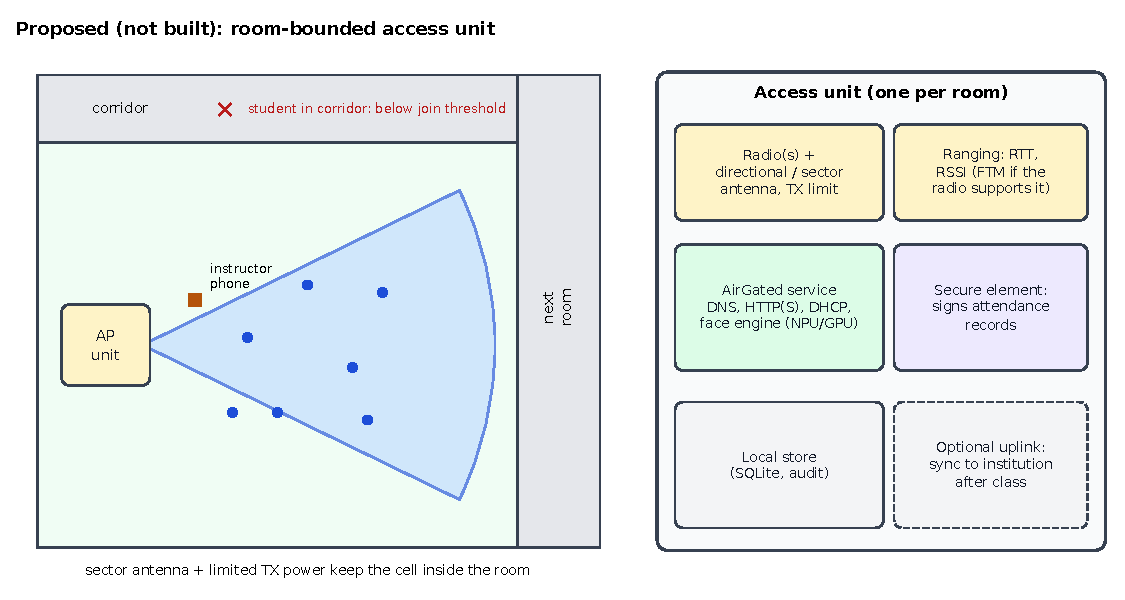
\includegraphics[width=0.95\linewidth]{figures/fig_hardware.pdf}
\caption{Concept (not built): a per-room unit with a sector antenna and limited transmit power keeps the cell inside the room; a student in the corridor falls below the join threshold. Right: functional blocks of the unit.}
\label{fig:hardware}
\end{figure}

\paragraph{Why hardware.} It addresses four findings at once: the client cap of consumer hotspots, the DNS and DHCP conflicts with operating-system services (the unit owns the network stack, satisfying H1--H5), the gateway requirement behind the MAC lookup, and the lack of a room-presence signal. An earlier plan considered an off-the-shelf dual-band router for the same reasons, including that 5~GHz attenuates faster through walls than 2.4~GHz; it was evaluated but never purchased or tested, and a custom unit generalises that idea.

\paragraph{Coverage control.} A sector or directional antenna and an adjustable transmit power can shape the cell so it fills the seating area rather than the corridor (Figure~\ref{fig:hardware}). Radio does not respect walls exactly, so each room needs a site survey, and the unit does not stop a second device carried into the room, which the key and face checks still catch. The posture is layered: radio containment as the primary presence boundary, the signed check-in pipeline underneath it, and a brief instructor spot check as a backstop. A received-signal-strength threshold and, where the radio supports fine timing measurement, time-of-flight ranging could add a measured presence signal to the gates; we have not tested either.

\paragraph{Capacity and compute.} The unit must support a whole class of associations (the target is a documented, measured client count above the class size, to be verified with the monitor tool and real phones) and must analyse face clips faster than one at a time: the measured 1.8~s serial analysis is the first limit seen. An accelerator or a parallel pipeline is needed, and analysis time per class should be a stated requirement.

\paragraph{Instructor on a phone.} Running a class from the instructor's phone requires an authenticated channel to the unit: the phone enrolled with its own non-extractable key and a face check, a role flag, and rate limiting, so that a student cannot reach the dashboard or reset enrollments. This replaces the present loopback-only rule.

\paragraph{Platform independence and trust.} The service should not depend on one vendor's firmware. The unit would run the same application on a small embedded Linux image, store records locally, and could sign attendance records with a key held in a secure element and optionally sync them to an institutional system after class. Per-room units would be managed by the institution administrator role of Section~\ref{sec:roles}. None of this is implemented.

\section{Conclusion}
\sys{} shows that a host on the classroom network can bind attendance to the phone (a non-extractable key), the person (a face-and-blink check) and the network (server-measured latency and link-layer address) without cloud services. Its defect history and its move from Windows to Linux show that most failures came from ordering and environment, and that the operating-system-specific surface is small: access-point creation, IP-to-MAC lookup and DNS start order. Treating a changed MAC as a re-registration trigger when key and face verify removes the main source of avoidable lost attendance. The system is still a prototype. The next work is liveness and threshold calibration, class-scale capacity measurement, authenticated instructor access from a phone, and a dedicated access unit that bounds coverage to one room.

\paragraph{Artifacts.} Source code, tests, the Linux launcher, hotspot script, monitor, load test and figure generator are in the repository at \url{https://github.com/unexperiencedone/airgated-}.

\paragraph{Disclosure.} The author designed the system, made the design decisions and tested it with real students and phones. Claude (Anthropic's AI coding assistant) was used to help write most of the code, tests and documentation, including this manuscript; the author is responsible for its content. Student identifiers and face images are omitted.

\begin{thebibliography}{9}
\bibitem{martin2017mac} J.~Martin, T.~Mayberry, C.~Donahue, L.~Foppe, L.~Brown, C.~Riggins, E.~C.~Rye, D.~Brown. A study of MAC address randomization in mobile devices and when it fails. \emph{Proceedings on Privacy Enhancing Technologies}, 2017(4):365--383, 2017.
\bibitem{webcrypto} W3C. Web Cryptography API. W3C Recommendation, 2017.
\bibitem{yunet} W.~Wu, H.~Peng, S.~Yu. YuNet: A tiny millisecond-level face detector. \emph{Machine Intelligence Research}, 2023.
\bibitem{sface} Y.~Zhong, W.~Deng, J.~Hu, D.~Zhao, X.~Li, D.~Wen. SFace: Sigmoid-constrained hypersphere loss for robust face recognition. \emph{IEEE Transactions on Image Processing}, 30:2587--2598, 2021.
\bibitem{mediapipe} C.~Lugaresi et al. MediaPipe: A framework for building perception pipelines. arXiv:1906.08172, 2019.
\end{thebibliography}

\end{document}
